%  !TeX  root  =  user_guide.tex  

%\section{eVis Plugin}\label{sec:evis}
\section{Extension eVis}\label{sec:evis}

%The Biodiversity Informatics Facility at the American Museum of Natural History's (AMNH) Center 
%for Biodiversity and Conservation (CBC) \footnote{This section is derived from Horning, N., K.
%Koy, P. Ersts. 2009. eVis (v1.1.0) User's Guide. American Museum of
%Natural History, Center for Biodiversity and Conservation. Available from
%\url{http://biodiversityinformatics.amnh.org/}, and released under the GNU FDL.} has developed the
%Event Visualization Tool (eVis), 
%another software tool to add to the suite of conservation monitoring and decision support tools 
%for guiding protected area and landscape planning. This plugin enables users to easily link 
%geocoded (i.e., referenced with latitude and longitude or X and Y coordinates) photographs, 
%and other supporting documents, to vector data in \qg.

Le laboratoire \og Biodiversity Informatics\fg du Centre pour la Conservation et la Biodiversité (CBC) du Musée américain d'Histoire Naturelle (AMNH) \footnote{Cette partie est tirée de Horning, N., K. Koy, P. Ersts. 2009. eVis (v1.1.0) User's Guide. American Museum of
Natural History, Center for Biodiversity and Conservation. Disponible à \url{http://biodiversityinformatics.amnh.org/}, est publié sous la licence GNU FDL.} a développé l'outil de visualisation des évènements (eVis) qui fait partit d'une suite logicielle destinée à la gestion et la surveillance des zones naturelles protégées. Cette extension permet à un utilisateur de lier facilement des photographies géocodées (c-à-d avec des coordonnées lat/long ou X/Y renseignées) et d'autres types de documents à des données vectorielles dans \qg.

%eVis is now automatically installed and enabled in new versions of \qg, and as with all plugins, 
%it can be disabled and enabled using the Plugin Manager (See Section \ref{sec:managing_plugins}).

eVis est dorénavant installé automatiquement dans les nouvelles versions de \qg, comme toutes les extensions elle peut être activé ou désactivé dans le gestionnaire d'Extension (voir section \ref{sec:managing_plugins}).

%The eVis plugin is made up of three modules: the Database Connection tool, Event ID tool, and 
%the Event Browser. These work together to allow viewing of geocoded photographs and other documents 
%that are linked to features stored in vector files, databases, or spreadsheets.

L'extension consiste en 3 modules : l'outil de connexion à une base de données, l'outil ID et le navigateur d'évènements. Ils fonctionnent ensemble pour permettre l'affichage de documents géoéréfrencés qui sont liés à des entités enregistrées dans des fichiers vectoriels, des bases de données ou des feuilles de tableur.

\subsection{Navigateur d'évènement}\label{evis_browser}
%\subsection{Event Browser}\label{evis_browser}

%The Event Browser module provides the functionality to display geocoded photographs that are linked
%to vector features displayed in the \qg map window. Point data, for example, can be from a vector
%file that can be input using \qg or it can be from the result of a database query. The vector
%feature must have attribute information associated with it to describe the location and name of the
%file containing the photograph and, optionally, the compass direction the camera was pointed when
%the image was acquired. Your vector layer must be loaded into \qg before running the Event Browser.

Le navigateur d'évènement fournit la capacité d'afficher des photographies ayant un lien avec les entités vecteurs affichées dans la fenêtre principale de \qg. Ces entités doivent avoir des informations attributaires associées décrivant l'emplacement et le nom du fichier contenant la photographie et, optionnellement, la direction vers laquelle était pointé l'objectif lors de la prise de l'image. Votre couche vectorielle doit être chargéedans \qg avant le lancement du navigateur d'évènements.

%\minisec{Launch the Event Browser module}\label{evis_launch_browser}
\minisec{Afficher le navigateur d'évènements}\label{evis_launch_browser}

%To launch the Event browser module either click on the \toolbtntwo{event_browser}{Event Browser}
%icon or click on \mainmenuopt{Plugins} > \dropmenuopt{eVis} >
%\dropmenuopt{eVis Event Browser}. This will open the Generic Event Browser window.

Pour lancer le navigateur d'évènements, vous pouvez soit cliquer sur l'icône\\ \toolbtntwo{event_browser}{Navigateur d'évènements} ou bien cliquer sur le menu \mainmenuopt{Extension} > \dropmenuopt{eVis} >\\ \dropmenuopt{navigateur d'évènements eVis}.

%The Generic Event Browser window has three tabs displayed at the top of the window. The Display tab
%is used to view the photograph and its associated attribute data. The Options tab provides a number
%of settings that can be adjusted to control the behavior of the eVis plugin. Lastly, the Configure
%External Applications tab is used to maintain a table of file extensions and their associated
%application to allow eVis to display documents other than images.

La fenêtre générique du navigateur affiche 3 onglets dans sa partie supérieure. L'onglet d'affichage est utilisé pour voir la photographie et les données attributaires correspondantes. L'onglet des options fournit une série de paramètres qui peuvent être ajustés pour contrôler le comportement de l'extension eVis. Enfin, l'onglet de configuration des applications externes contient une table des extensions de fichiers et des applications qui leur sont associées pour permettre à eVis d'afficher des documents autre qu'une image.

%\minisec{Understanding the Display window}\label{evis_display_window}
\minisec{Comprendre la fenêtre d'affichage}\label{evis_display_window}

%To see the Display window click on the \tab{Display} tab in the Generic Event Browser
%window. The Display window is used to view geocoded photographs and their associated attribute data.
Pour la voir, cliquez sur l'onglet \tab{Affichage} du navigateur d'évènements. Cette fenêtre est utilisée pour regarder les photographies et leurs données attributaires.

%\begin{figure}[ht]
%   \begin{center}
%\caption{\label{evisdisplay}The \emph{eVis} display window \nixcaption}
%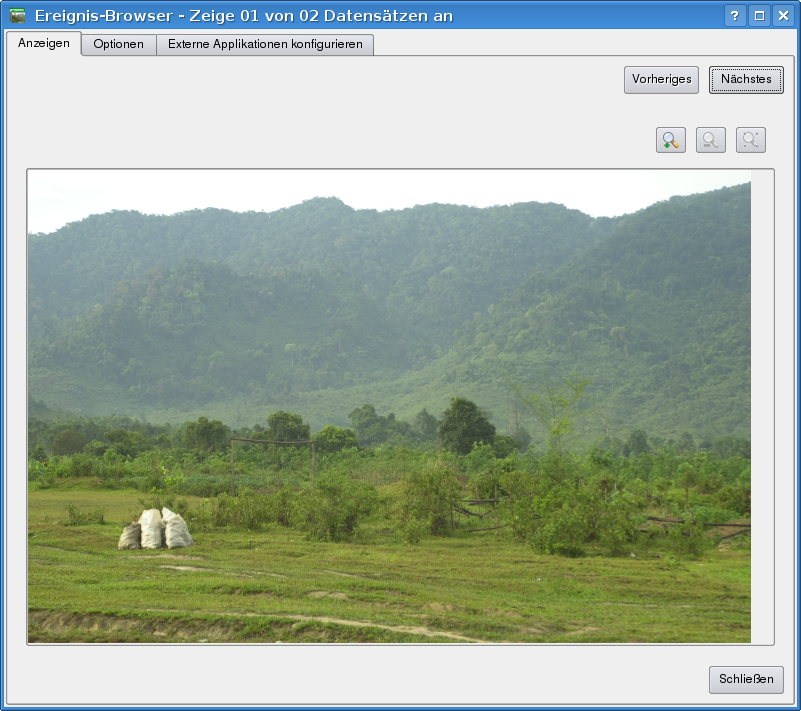
\includegraphics[clip=true, width=12cm]{evisdisplay}
%\end{center}
%\end{figure}
\begin{figure}[ht]
   \begin{center}
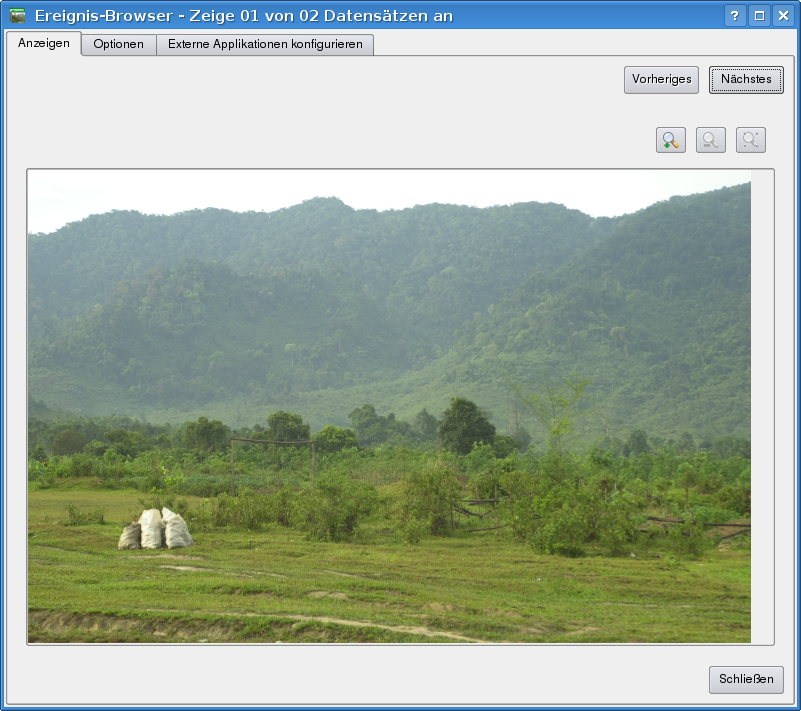
\includegraphics[clip=true, width=10cm]{evisdisplay}
\caption{\label{evisdisplay}La fenêtre d'affichage \emph{eVis} \nixcaption}
\end{center}
\end{figure}

%\begin{itemize}
%\item \textbf{Display window :] A window where the photograph will appear.
%\item \textbf{Increase zoom button :] Zoom in to see more detail. If the entire image cannot be
%displayed in the display window, scroll bars will appear on the left and bottom sides of the window
%to allow you to pan around the image.
%\item \textbf{Reduce zoom button :] Zoom out to see more area. 
%\item \textbf{Zoom to full extent button :] Displays the full extent of the photograph.
%\item \textbf{Attribute information window :] All of the attribute information for the point
%associated with the photograph being viewed is displayed here. If the file type being referenced in
%the displayed record is not an image but is of a file type defined in the Configure External
%Applications tab then when you double-click on the value of the field containing the path to the
%file the application to open the file will be launched to view or hear the contents of the file. If
%the file extension is recognized the attribute data will be displayed in green.
%\item \textbf{Navigation buttons :] Use the Previous and Next buttons to load the previous or next
%feature when more than one feature is selected.
%\item \textbf{Feature indicator :] This heading indicates which feature is being displayed and how
%many features are available for display.
%\end{itemize}

\begin{description}
\item[Zone d'affichage :] emplacement où s'affichera l'image.
\item[bouton d'augmentation du zoom :] Zoomez pour voir plus de détails. Si l'image entière ne peut être affichée dans la fenêtre, des barres de défilement apparaîtront sur les bords gauches et inférieures pour que vous puissiez bouger l'image.
\item[bouton de réduction du zoomn :] Zoomez en arrière pour avoir une vue d'ensemble.
\item[bouton pour zoomer sur l'emprise :] Affiche l'emprise maximale de la photographie.
\item[Zone d'informations :] Toutes les informations attributaires pour le point associé à la photographie sélectionnée sont affichées ici. Si le type de fichier référencé n'est pas une image, mais d'un type renseigné dans la liste des applications externe (il sera alors affiché en vert), un double clic lancera l'application désignée.
\item[boutons de navigation :] Utilisez les boutons Suivant et Précédent pour charger une autre entité lorsque  plusieurs sont sélectionnées.
\item[Indicateur d'entité :] Cet en-tête indique quelle entité est affichée et combien d'entités sont disponibles pour l'affichage.
\end{description}

%\minisec{Understanding the Options window}\label{evis_options_window}
\minisec{Comprendre la fenêtre des options}\label{evis_options_window}

%\begin{figure}[ht]
%   \begin{center}
%\caption{\label{evisoptions}The \emph{eVis} Options window \nixcaption}
%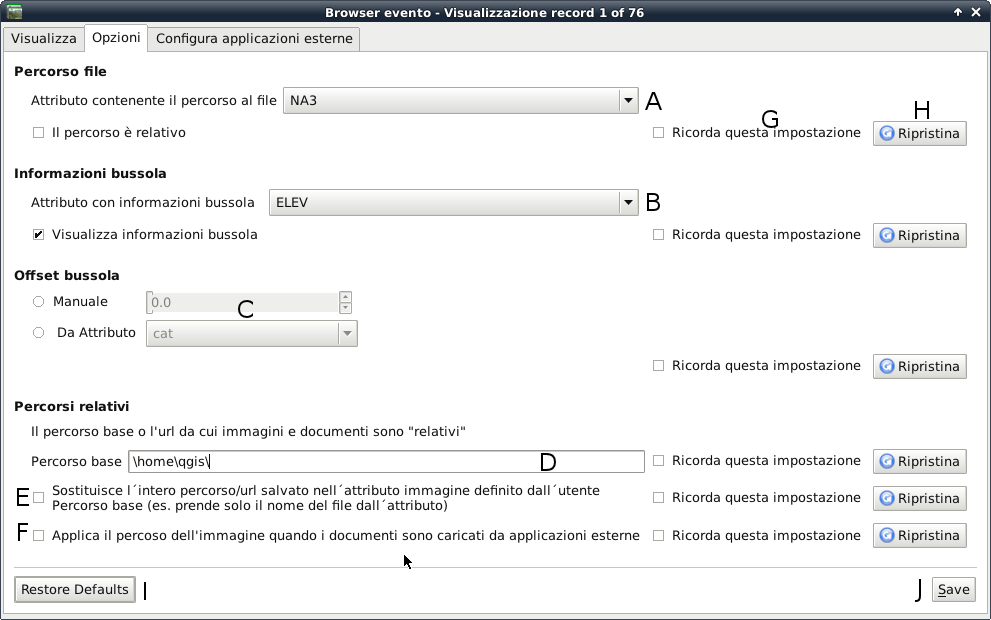
\includegraphics[clip=true, width=12cm]{evisoptions}
%\end{center}
%\end{figure}
\begin{figure}[ht]
   \begin{center}
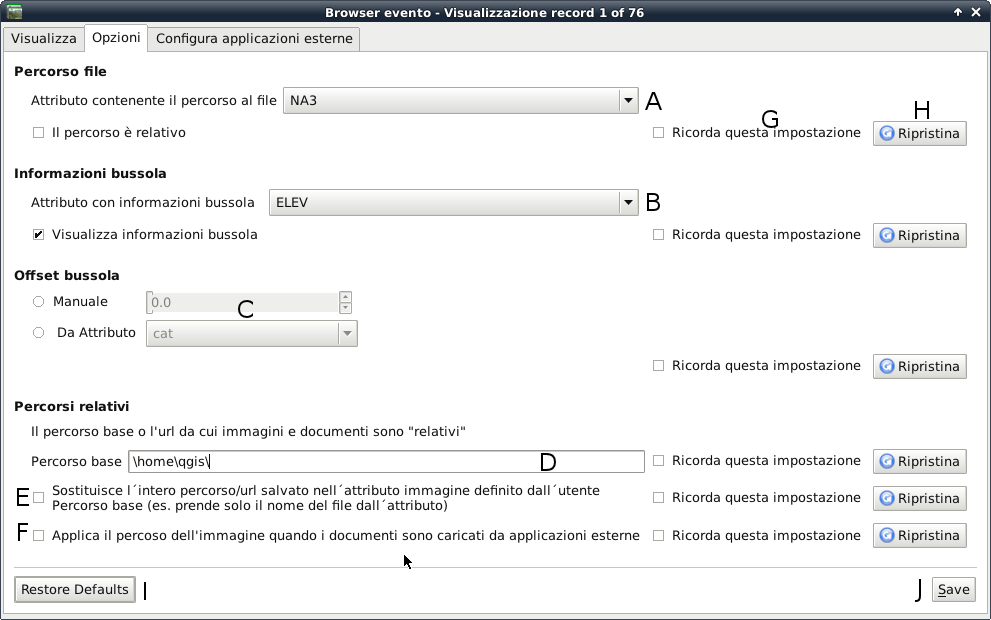
\includegraphics[clip=true, width=10cm]{evisoptions}
\caption{\label{evisoptions}fenêtre des options de \emph{eVis} \nixcaption}
\end{center}
\end{figure}

%\begin{itemize}
%\item[File location :] A dropdown list to specify the attribute field that contains the
%directory path or URL for the photographs or other documents being displayed. If the location is a
%relative path then the checkbox to the right of the dropdown menu must be clicked. The base path for
%a relative path can be entered in the Base Path text box below. Information about the different
%options for specifying the file location are noted in the section 4.5 below.
%\item[Compass bearing display field :] A dropdown list to specify the attribute field
%that contains the compass bearing associated with the photograph being displayed. If compass bearing
%information is available it is necessary to click the radio button to the left of the dropdown menu
%title.
%\item[Compass offset setting :] Compass offsets can be used to compensate for
%declination (adjust bearings collected using magnetic bearings to true north bearings). Click the
%Manual radio-button to enter the offset in the text box or click the From Attribute  radio-button to
%select the attribute field containing the offsets. For both of these options east declinations
%should be entered using positive values and west declinations should use negative values.
%\item[Directory base path :] The base path onto which the relative path defined in
%Figure \ref{evisoptions} (A) will be appended.
%\item[Replace path :] If this check-box is checked, only the file name from the A
%will be appended to the Base Path.
%\item[Apply rule to all documents :] If checked, the same path rules that are defined
%for photographs will be used for non-image documents such as movies, text documents, and sound
%files. If not checked the path rules will only apply to photographs and other documents will ignore
%the Base Path  parameter.
%\item[Save settings :] If the check-box is checked the values for the associated
%parameters will be saved for the next session when the window is closed or when the Save button
%below is pressed.
%\item[Reset values :] Resets the values on this line to the default setting.
%\item[Restore faults :] This will reset all of the fields to their default settings.
%It has the same effect as clicking all of the Reset buttons.
%\item[Save :] This will save the settings without closing the Options pane.
%\end{itemize}

\begin{description}
\item[Chemin du fichier :] Une liste déroulante permet de spécifier quel est l'attribut contenant le chemin d'accès vers le document devant être affiché. Si l'emplacement est un chemin relatif alors la boîte à cocher juste en dessous doit être activée. Le chemin de base peut être saisi dans la zone de texte. Les informations à propos des différentes options pour indiquer le chemin sont expliquées dans une section suivante.
\item[Attribut contenant le compas :] Une liste déroulante permet de spécifier le champ contenant les informations sur l'orientation de la photographie affichée. Si cette information est disponible, il est indispensable de cliquer sur la boîte à cocher situé à gauche de la liste.
\item[Décalage du compas :] Ce décalage peut être utilisé pour compenser une déclinaison (pour passer du nord magnétique au nord géographique) Cliquez sur le bouton Manuel pour le saisir  ou cliquez sur Depuis l'Attribut pour sélectionner le champ attributaire contenant cette indication. Dans elss 2 cas, la déclinaison Est doit être une valeur positive tandis que la déclinaison Ouest doit être négative.
\item[Chemin de base :] C'est le chemin à partir duquel le chemin relatif (A) définit dans la figure \ref{evisoptions} sera établi.
\item[Remplacer le chemin :] Si cette case est cochée alors uniquement le nom du fichier sera ajouté au chemin de base.
\item[Appliquer la règle à tous les documents :] Si cochée, la règle définie pour les photographies sera utilisée pour les autres documents tels que les vidéos et les fichiers audio.
\item[Ce souvenir de :] Si cette case est cochée, les valeurs des paramètres correspondants seront enregistrées pour la prochaine session.
\item[Réinitialiser :] Remet les valeurs par défaut pour ce paramètre.
\item[Restorer les valeurs par défaut :] Restore tout les paramètres par défaut.
\item[Enregsitrer :] Ceci enregistrera les valeurs sans fermer l'onglet des options.
\end{description}

%\minisec{Understanding the Configure External Applications window}\label{evis_external_window}
\minisec{Comprendre la fenêtre des Applications externes}\label{evis_external_window}

%\begin{figure}[htp]
%   \begin{center}
%\caption{\label{evisexternal}The \emph{eVis} External Applications window \nixcaption}
%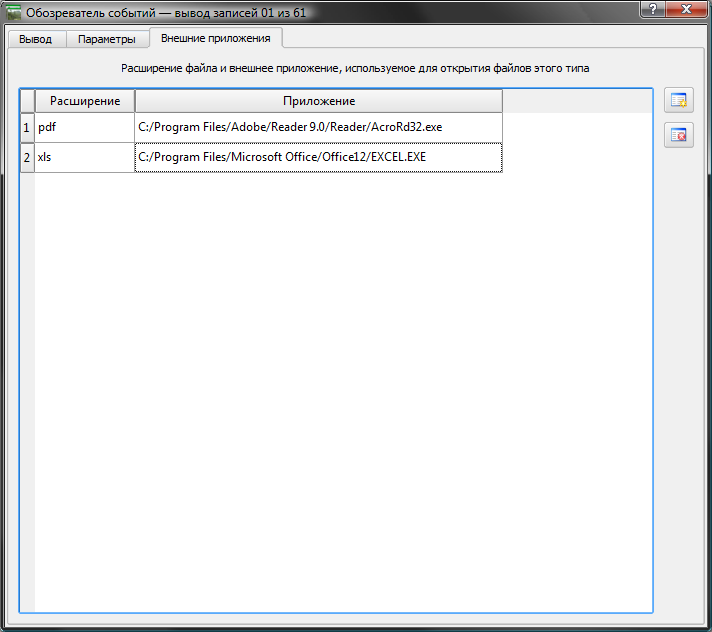
\includegraphics[clip=true, width=12cm]{evisexternal}
%\end{center}
%\end{figure}
\begin{figure}[htp]
   \begin{center}
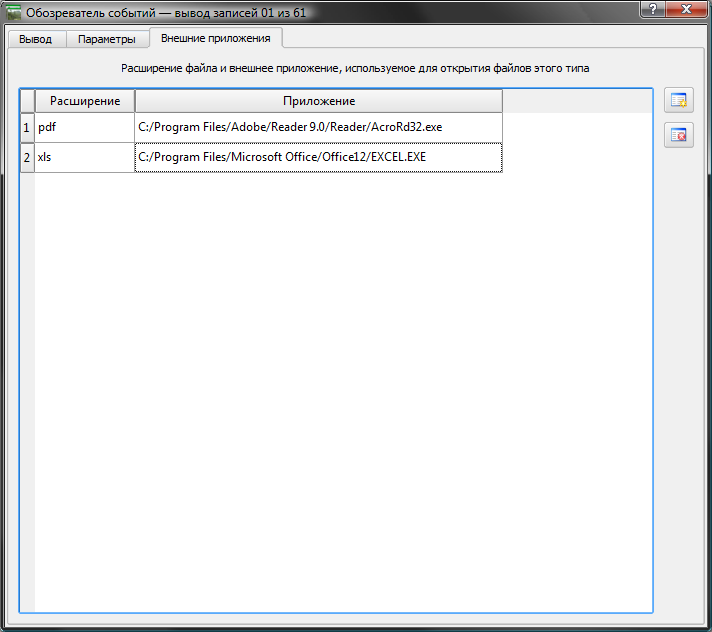
\includegraphics[clip=true, width=12cm]{evisexternal}
\caption{\label{evisexternal}Fenêtre des Applications externes \emph{eVis} \nixcaption}
\end{center}
\end{figure}

%\begin{itemize}
%\item[File reference table :] A table containing file types that can be opened using eVis.
%Each file type needs a file extension and the path to an application that can open that type of
%file. This provides the capability of opening a broad range of files such as movies, sound
%recordings, and text documents instead of only images.
%\item[Add new file type :] Add a new file type with a unique extension and the path
%for the application that can open the file.
%\item[Delete current row :] Delete the file type highlighted in the table and defined
%by a file extension and a path to an associated application.
%\end{itemize}

\begin{description}
\item[tableau des références :] Une table contient tous les types de fichiers qui peuvent être ouvert par eVis. Chaque type de fichier doit avoir une extension qui lui soit propre et un chemin vers une application pour l'ouvrir. Ce la permet d'utiliser un large éventail de documents autre que des images.
\item[Ajouter un nouveau type de fichier :] Ajout d'un nouveau type de fichier avec son extension et une application dédiée.
\item[Effacer la cellule courante :] Effacer le type de fichier sélectionné dans la table.
\end{description}

%\minisec{Specifying the location and name of a photograph}\label{evis_specifying}
\minisec{Spécifier un emplacement et le nom d'une photographie}\label{evis_specifying}

%The location and name of the photograph can be stored using an absolute or relative path or a URL if
%the photograph is available on a web server. Examples of the different approaches are listed in
%Table \ref{tab:evis_examples}.

Le nom et l'emplacement d'une photographie peuvent être enregistrés avec un chemin absolu ou relatif ou une URL si l'image se trouve sur un serveur Internet. Des exemples de ces différentes approches sont listés dans la table \ref{tab:evis_examples}.

%\begin{table}[htp]\label{tab:evis_examples}\index{extension!evis}
%\centering
%\caption{Example format using absolute path, relative path, and a
%URL}\medskip
% \begin{tabular}{|p{0.55in}|p{0.55in}|p{4.7in}|p{0.7in}|}
% \hline \textbf{X} & \textbf{Y} & \textbf{FILE} & \textbf{BEARING}\\
% \hline 780596 & 1784017 & \filename{C:\textbackslash Workshop\textbackslash
%eVis\_Data\textbackslash groundphotos\textbackslash DSC\_0168.JPG} & 275\\
% \hline 780596 & 1784017 & \filename{/groundphotos/DSC\_0169.JPG} & 80\\
% \hline 780819 & 1784015 &
%\filename{http://biodiversityinformatics.amnh.org/evis\_test\_data/DSC\_0170.JPG} & 10\\
% \hline 780596 & 1784017 & \filename{pdf:http://www.testsite.com/attachments.php?attachment\_id-12}
%& 76\\
% \hline
%\end{tabular}
%\end{table}
\begin{table}[htp]\label{tab:evis_examples}\index{extension!evis}
\centering
 \begin{tabular}{|p{1.5cm}|p{1.5cm}|p{8.5cm}|p{1.5cm}|}
 \hline \textbf{X} & \textbf{Y} & \textbf{FICHIER} & \textbf{BEARING}\\
 \hline 780596 & 1784017 & \filename{C:\textbackslash Workshop\textbackslash
eVis\_Data\textbackslash groundphotos\textbackslash DSC\_0168.JPG} & 275\\
 \hline 780596 & 1784017 & \filename{/groundphotos/DSC\_0169.JPG} & 80\\
 \hline 780819 & 1784015 &
\filename{http://biodiversityinformatics.amnh.org/}\par\filename{evis\_test\_data/DSC\_0170.JPG} & 10\\
 \hline 780596 & 1784017 & \filename{pdf:http://www.testsite.com/attachments.php?}\par\filename{attachment\_id-12}
& 76\\
 \hline
\end{tabular}
\caption{Exemple de chemin absolut, relatif et internet}
\end{table}

%\minisec{Specifying the location and name of a other supporting
%documents}\label{evis_location}
\minisec{Spécifier l'emplacement et le nom d'un document autre qu'image}\label{evis_location}

Les documents texte, vidéos ou audio peuvent aussi être affiché ou accéder par eVis. pour ce faire il est nécessaire d'ajouter une entrée dans la table des références fichiers qui pourra être utilisé par l'une des applications externes définies. Il est aussi nécessaire d'avoir le chemin vers le fichier dans la table attributaire de la couche vectorielle. Une possibilité supplémentaire est de spécifier l'extension du fichier avant le chemin (avi:/chemin/du/fichier), ce qui est très utile pour accéder à des documents placés sur des sites ou des wiki utilisant une base de données pour la gestion de leurs pages (voir la table \ref{tab:evis_examples}).

%\minisec{Using the Generic Event Browser}\label{evis_using_browser}
\minisec{Using the Generic Event Browser}\label{evis_using_browser}

%When the Event Browser window opens a photograph will appear in the display window if the document
%referenced in the vector file attribute table is an image and if the file location information in
%the Options window is properly set. If a photograph is expected and it does not appear it will be
%necessary to adjust the parameters in the Options window.

Quand la fenêtre du navigateur d'évènements s'ouvre, une photographie apparaîtra dans l'onglet d'affichage si le document référencé dans la table attributaire du fichier vectoriel est une image et que les paramètres d'emplacement sont correctement renseignés. Si la photographie voulue n'apparaît pas, c'est qu'il vous est nécessaire d'ajuster les paramètres de l'onglet des options.

%If a supporting document (or an image that does not have a file extension recognized by eVis) is
%referenced in the attribute table the field containing the file path will be highlighted in green in
%the attribute information window if that file extension is defined in the file reference table
%located in the Configure External Applications window. To open the document double-click on the
%green-highlighted line in the attribute information window. If a supporting document is referenced
%in the attribute information window and the file path is not highlighted in green then it will be
%necessary to add an entry for the file's filename extension in the Configure External Applications
%window. If the file path is highlighted in green but does not open when double-clicked it will be
%necessary to adjust the parameters in the Options window so the file can be located by eVis.

Si un document supporté (ou une image n'ayant pas d'extension reconnue par eVis) est référencé dans la table attributaire, le champ contenant le chemin vers le fichier sera surligné en vert dans la liste des références fichiers si cette extension a été définie dans la table de configuration des applications externes. Pour l'ouvrir, faites un double-clic sur la ligne en vert. Si un document est référencé, mais nonsurligné en vert, il est nécessaire d'ajouter une entrée pour son extension. Si le chemin est bien surligné en vert, mais qu'un double-clic reste sans effet, il faudra alors vérifier que l'application associée à l'extension est bien renseignée.

%If no compass bearing is provided in the Options window a red asterisk will be displayed on top of
%the vector feature that is associated with the photograph being displayed.
%If a compass bearing is provided then an arrow will appear pointing in the direction indicated by
%the value in the compass bearing display field in the Generic Event Browser window. The arrow will
%be centered over the point that is associated with the photograph or other document.

Si aucune indication de compas n'est fournie dans les options, un astérisque rouge sera affiché au-dessus de l'entité vectorielle concernée par l'image affichée. Si cette indication est disponible alors une flèche pointant la direction de l'objectif apparaîtra.

%To close the Generic Event Browser window click on the Close button from the Display window.
Pour fermer ce navigateur, cliquez sur le bouton Fermer de l'onglet d'affichage.

\subsection{l'outil ID}\label{evis_id_tool}

%The Event ID module allows you to display a photograph by clicking on a feature displayed in the
%\qg map window. The vector feature must have attribute information associated with it to describe
%the location and name of the file containing the photograph and optionally the compass direction the
%camera was pointed when the image was acquired. This layer must be loaded into \qg before running
%the Event ID tool.
L'outil ID d'évènement permet d'afficher une photographie en cliquant sur l'entité affichée dans la fenêtre de \qg. La couche vectorielle doit avoir des attributs associés indiquant l'emplacement et le nom du fichier. Cette couche doit être chargée avant d'utiliser cet outil.
\subsection{l'outil ID}\label{evis_id_tool}

%The Event ID module allows you to display a photograph by clicking on a feature displayed in the
%\qg map window. The vector feature must have attribute information associated with it to describe
%the location and name of the file containing the photograph and optionally the compass direction the
%camera was pointed when the image was acquired. This layer must be loaded into \qg before running
%the Event ID tool.
L'outil ID d'évènement permet d'afficher une photographie en cliquant sur l'entité affichée dans la fenêtre de \qg. la couche vectorielle doit avoir des attributs associés indiquant l'emplacement et le nom du fichier. Cette couche doit être chargée avant d'utiliser cet outil.

%\minisec{Launch the Event ID module}\label{evis_launch_id}
\minisec{Lancer le module ID}\label{evis_launch_id}

%To launch the Event ID module either click on the \toolbtntwo{event_id}{Event ID}
%icon or click on \mainmenuopt{Plugins} > \dropmenuopt{eVis} >
%\dropmenuopt{Event ID Tool}. This will cause the cursor to change to an arrow with an``i\fg  on top of
%it signifying that the ID tool is active.

Pour executer cet outil, cliquez sur l'icône \toolbtntwo{event_id}{Event ID} ou bien sur le menu \mainmenuopt{Extensions} > \dropmenuopt{eVis} > \dropmenuopt{Event ID Tool}. Cela provoquera le changement du curseur en une flèche avec un ``i\fg   à son sommet signifiant que l'outil ID est actif.

%To view the photographs linked to vector features in the active vector layer displayed in the \qg
%map window, move the Event ID cursor over the feature and then click the mouse. After clicking on
%the feature, the Generic Event Browser window is opened and the photographs on or near the clicked
%locality are available for display in the browser. If more than one photograph is available, you can
%cycle through the different features using the Previous and Next buttons. The other controls are
%described in the Event Browser section of this guide.

Pour visonner les photographies liées aux entitées de la couche vectorielle active, déplacez le curseur sur l'une d'elles et faites un clic. La fenêtre du navigateur d'évènements s'ouvre alors en affichant la photographie du point ou proche. Si plus d'une est disponible, vous pouvez faire défiler les différentes entités avec les bouons Suivant et Précédent.

%\subsection{Database connection}\label{evis_database}
\subsection{Connexion à une base de données}\label{evis_database}

%The Database Connection module provides tools to connect to and query a database or other ODDBC
%resource, such as a spreadsheet.

Cet outil permet de se connecter et d'interroger une base de données ou une ressource ODBC telle qu'un tableur.

%eVis can directly connect to four types of databases: Microsoft Access, PostgreSQL, MySQL, SQLITE,
%and can also read from ODBC connections. When reading from an ODBC database (such as an Excel
%spreadsheet) it is necessary to configure your ODBC driver for the operating system you are using.

eVis peut directement se connecter à 4 types de bases : Microsoft Access, PostgreSQL, MySQL, SQLITE. Il est possible de lire une connexion ODBC telle qu'une feuille Excel, dans ce cas il faut configurer cette connexion via votre système d'exploitation.

%\minisec{Launch the Database Connection module}\label{evis_launch_database}
\minisec{Lancer l'outil de connexion à une base de données}\label{evis_launch_database}

%To launch the Database Connection module either click on the appropriate icon
%\toolbtntwo{evis_connect}{} or click on \mainmenuopt{Plugins} > \dropmenuopt{eVis} >
%\dropmenuopt{Database Connection}. This will launch the Database Connection window. The window has
%three tabs: \tab{Predefined Queries}, \tab{Database Connection}, and \tab{SQL Query}. The Output
%Console window at the bottom of the window displays the status of actions initiated by the different
%sections of this module.

Cliquez sur l'icône \toolbtntwo{evis_connect}{} ou sur le menu \mainmenuopt{Extensions} > \dropmenuopt{eVis} >\\ \dropmenuopt{connexion à une base de données}. Cela ouvrira une fenêtre avec 3 onglets :\\ \tab{Requêtes prédéfinies}, \tab{Connexion à une base}, et \tab{Requête SQL}. La console de sortie en bas de la fenêtre affiche le statut des actions initialisées par les différentes sections de cet outil.

%\minisec{Connect to a database}\label{evis_connect_database}
\minisec{Se connecter à une base}\label{evis_connect_database}

%Click on the \tab{Database Connection} tab to open the database connection interface. Next, click on
%the \dropmenuopt{Database Type} dropdown menu to select the type of database that you want to
%connect to. If a password or username is required, that information can be entered in the Username
%and Password textboxes.

Cliquez sur l'onglet \tab{Connexion à une base} puis sur le menu déroulant\\ \dropmenuopt{Type de la base de données} pour sélectionner le type de base à laquelle vous voulez vous connecter. Vous pouvez saisir un nom d'utilisateur et un mot de passe si nécessaire.

%Enter the database host in the Database Host textbox. This option is not available if you selected
%\og MSAccess\fg  as the database type. If the database resides on your desktop you should enter
%\og localhost.\fg 

Entrez le nom de l'hôte de la base, cette option n'est pas disponible si vous avez sélectionné \og MSAccess\fg  comme type. Si la base de données est sur votre ordinateur, vous devrez saisir \og localhost.\fg .

%Enter the name of the database in the Database Name textbox. If you selected \og ODBC\fg  as the
%database type, you need to enter the data source name.

Entrez le nom de la base dans la zone de saisie correspondante. Si vous avez sélectionné \og ODBC\fg  comme type de base, vous devrez indiquer le nom de la source de données.

%When all of the parameters are filled in, click on the Connect button. If the connection is
%successful, a message will be written in the Output Console window stating that the connection was
%established. If a connection was not established you will need to check that the correct parameters
%were entered above.

Quand tout les paramètres sont corrects, cliquez sur le bouton Connecter. Si la connexion est réussie, un message sera écrit dans la console de sortie. En cas d'échec, il vous faudra vérifier les paramètres.

\begin{figure}[ht]
   \begin{center}
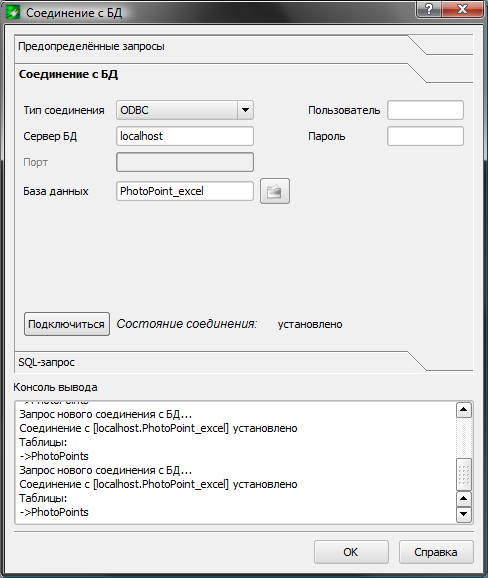
\includegraphics[clip=true, width=8cm]{evisdatabase}
\caption{\label{evisdatabase}Fenêtre de connexion à une base de données \emph{eVis} \nixcaption}
\end{center}
\end{figure}

\begin{description}
\item[Type de base de données :] Une liste déroulante pour spécifier le type de base utilisée.
\item[Hôte de la base de données :] le nom de l'hôte de la base.
\item[Port :] Le chiffre du port dans le cas d'une base \og MYSQL\fg .
\item[Nom de la base de données :] The name of the database.
\item[Connecter :] Ce bouton établit la connexion avec les paramètres définis.
\item[Console de sortie :] Console où sont affichés les messages relatifs au déroulement de la connexion.
\item[Nom d'utilisateur :] Nécessaire quand la base est protégée en accès.
\item[Mot de passe :] Nécessaire quand la base est protégée en accès.
\item[Requêtes Prédéfinies :]  Onglet ouvrant la fenêtre de \og Requêtes Prédéfinies\fg .
\item[Connexion à une base de données :] Onglet ouvrant la fenêtre de \og Connexion à une base de données\fg .
\item[Requête SQL :] Onglet ouvrant la fenêtre de \og Requête SQL\fg .
\item[Aide :] Affiche l'aide en ligne.
\item[OK :] Ferme la fenêtre \og Connexion à une base de données\fg .
\end{description}

%\minisec{Running SQL queries}\label{evis_running_sql}
\minisec{Faire une requête SQL}\label{evis_running_sql}

%SQL queries are used to extract information from a database or ODBC resource. In eVis the output
%from these queries is a vector layer added to the \qg map window. Click on the \tab{SQL Query} tab
%to display the SQL query interface. SQL commands can be entered in this text window. A helpful
%tutorial on SQL commands is available at \url{http://www.w3schools.com/sql/}. For example, to
%extract all of the data from a worksheet in an Excel file, \og select * from [sheet1\$]\fg 
%where\og sheet1\fg  is the name of the worksheet.

Les requêtes SQL sont utilisées pour extraire des informations depuis une base de données ou unesource ODBC. Dans eVis, le résultat de ces requêtes est une couche vectorielle ajoutée à \qg. cliquez sur l'onglet \tab{Requête SQL} pour afficher l'interface. Les commandes SQL peuvent être saisies depuis cette fenêtre de texte. Un tutoriel bien pratique sur les commandes SQl est disponible à \url{http://www.w3schools.com/sql/}. Par exemple, pour extraire toutes les données d'un fichier Excel, faites\og select * from [sheet1\$]\fg  où \og sheet1\fg  est le nom de la feuille concernée.
where\og sheet1\fg .

%Click on the Run Query button to execute the command. If the query is successful a Database File
%Selection window will be displayed. If the query is not successful an error message will appear in
%the Output Console widow.

Cliquez sur le bouton Exécuter la requête pour exécuter la commande. Si la requête est fructueuse, une fenêtre de sélection sera affichée. Dans le cas contraire, un message d'erreur apparaîtra dans la console de sortie.

%In the Database File Selection window, enter the name of the layer that will be created from the
%results of the query in the Name of New Layer textbox.

Dans cette nouvelle fenêtre, entrez le nom de la couche qui sera créée à partir des résultats dans la zone de texte Nom de la Nouvelle Couche.

%\begin{figure}[ht]
%   \begin{center}
%\caption{\label{evissql_query}The \emph{eVis} SQL query tab \nixcaption}
%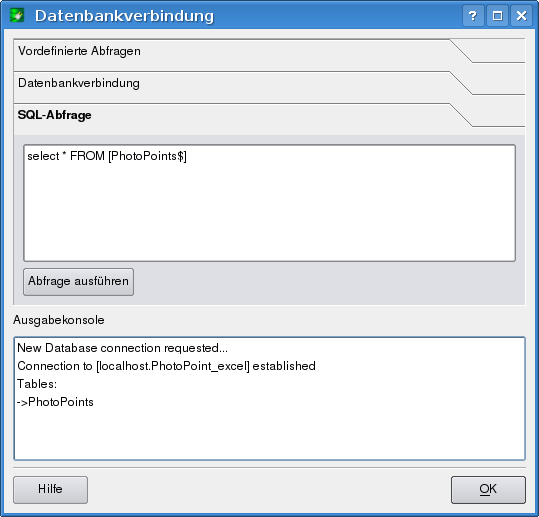
\includegraphics[clip=true, width=12cm]{evissql_query}
%\end{center}
%\end{figure}
\begin{figure}[ht]
   \begin{center}
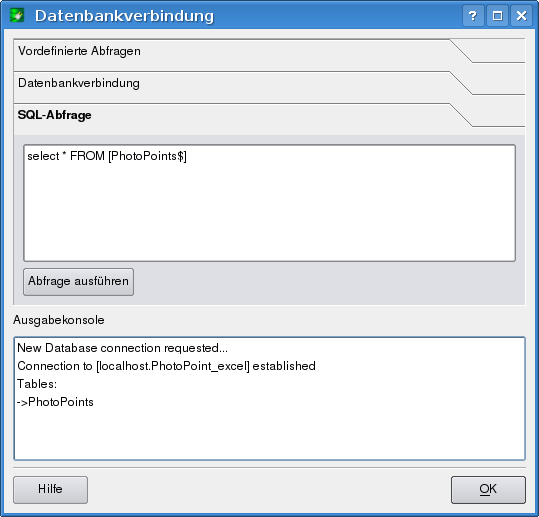
\includegraphics[clip=true, width=8cm]{evissql_query}
\caption{\label{evissql_query}L'onglet de requête SQL \emph{eVis} \nixcaption}
\end{center}
\end{figure}

%\begin{itemize}
%\item[SQL Query Text Window :] A screen to type SQL queries.
%\item[Run Query :] Button to execute the query entered in the SQL Query Window.
%\item[Console Window :] The console window where messages related to processing are
%displayed.
%\item[Help :] Displays the on line help.
%\item[OK :] If this check-box is checked, only the file name from the A will be appended to
%the Base Path.
%\item[Apply rule to all documents :] Closes the main \og Database Connection\fg  window.
%\end{itemize}
\begin{description}
\item[Zone de texte de requête SQL :] Une zone poursaisir vos requêtes
\item[exécuter la requête :] Ce bouton exécute la requête écrite.
\item[Console :] Console où sont affichés les messages relatifs au déroulement de la connexion.
\item[Aide :] Affiche l'aide en ligne.
\item[OK :] Si cette case est cochée, seul le nom du fichier sera ajouté au chemin de base.
\item[Appliquer la règle tous les documents :] Ferme la fenêtre principale \og Connexion à une base de données\fg .
\end{description}

%Use the \dropmenuopt{X Coordinate} and \dropmenuopt{Y Coordinate} dropdown menus to select the field
%from the database that store the \og X\fg  (or longitude) and \og Y\fg  (or latitude) coordinates. Clicking
%on the OK button causes the vector layer created from the SQL query to be displayed in the \qg map
%window.

Utilisez les menus déroulants \dropmenuopt{Coordonnée X} et \dropmenuopt{Coordonnée Y} pour choisir les champs stockant les coordonnées en \og X\fg  (ou longitude) et \og Y\fg  (ou latitude). Cliquez sur Ok pour créer la couche vectorielle qui sera affichée sur la carte de \qg.

%To save this vector file for future use, you can use the \qg \og Save as shapefile\fg  command that is
%accessed by right clicking on the layer name in the \qg map legend and then selecting \og Save as
%shapefile.\fg 

Pour enregistrer ce fichier pour une utilisation ultérieure, vous pouvez utiliser la fonction de \qg \og Sauvegarder comme shapefile\fg  accessible via un clic droit sur la couche listée dans la zone de légende.

%\begin{Tip}\caption{\textsc{Creating a vector layer from a Microsoft Excel Worksheet}}
%\qgistip{When creating a vector layer from a Microsoft Excel Worksheet you might see that unwanted
%zeros (\og 0\fg ) have been inserted in the attribute table rows beneath valid data.This can be caused
%by deleting the values for these cells in Excel using the \og backspace\fg  key. To correct this problem
%you need to open the Excel file (you'll need to close \qg if there if you are connected to the file
%to allow you to edit the file) and then use Edit > Delete to remove the blank rows from the file. To
%avoid this problem you can simply delete several rows in the Excel Worksheet using Edit > Delete
%before saving the file.}
%\end{Tip}

\begin{Tip}\caption{\textsc{Créer une couche vectorielle depuis un fichier Microsoft Excel}}
Lorsque vous créer une couche vectorielle depuis un fichier Excel, vous risquez peut être de voir des zéros (\og 0\fg ) insérés dans les lignes de la table attributaire à l a suite de données valides. Cela peut être causé par l'utilisation de la touche \og Entrée\fg dans une cellule. pour corriger ce problème, vous devez ouvrir le fichier (après avoir fermé \qg si vous y êtes connecté) et utiliser le menu Édition > Effacer le contenu pour supprimer les espaces blancs.
\end{Tip}

%\minisec{Running predefined queries}\label{evis_predefined}
\minisec{Exécuter des requête prédéfinies}\label{evis_predefined}

%With predefined queries you can select previously written queries stored in XML format in a file.
%This is particularly helpful if you are not familiar with SQL commands. Click on the \tab{Predefined
%Queries} tab to display the predefined query interface.

Avec les requêtes prédéfinies, vous pouvez sélectionner des requêtes déjà écrites et stockées au format XML. Cela peut être utile si vous n'êtes pas familier avec les commandes SQL. Cliquez sur l'onglet \tab{requête prédéfinies} pour afficher l'interface.

%To load a set of predefined queries click on the \toolbtntwo{evis_file}{Open File} icon. This opens
%the Open File window which is used to locate the file containing the SQL queries. When the queries
%are loaded their titles, as defined in the XML file, will appear in the dropdown menu located just
%below the \toolbtntwo{evis_file}{Open File} icon, the full description of the query is displayed in
%the text window under the dropdown menu.

Pour charger un jeu de requêtes prédéfinies, cliquez sur l'icône \toolbtntwo{evis_file}{Open File}. Une fenêtre s'ouvre pour sélectionner le fichier. Lorsque les requêtes sont chargées, leurs titres définis au format XML apparaîtront dans le menu déroulant situé en dessous de l'icône \toolbtntwo{evis_file}{Open File}, la description complète de la requête est affichée dans la zone en dessous de la liste.

%Select the query you want to run from the dropdown menu and then click on the SQL Query tab to see
%that the query has been loaded into the query window. If it is the first time you are running a
%predefined query or are switching databases, you need to be sure to connect to the database.

Sélectionnez la requête que vous voulez exécuter depuis la liste déroulante et ensuite cliquez sur l'onglet de requête SQL pour observer la requête qui vient d'être chargée. Si c'est la première fois que vous exécutez une requête prédéfinie ou que vous changez de base de travail, vous devrez vous connecter à la base de données.

%Click on the \button{Run Query} button in the \tab{SQL Query} tab to execute the command. If the
%query is successful a Database File Selection window will be displayed. If the query is not
%successful an error message will appear in the Output Console window.

Cliquez sur le bouton \button{Exécuter la requête} dans l'onglet \tab{Requête SQL} pour lancer la commande. Si la requête est fructueuse, une fenêtre de sélection sera affichée. Dans le cas contraire, un message d'erreur apparaîtra dans la console de sortie.

%\begin{figure}[htp]
%   \begin{center}
%\caption{\label{evispredefined}The \emph{eVis} Perdefined queries tab \nixcaption}
%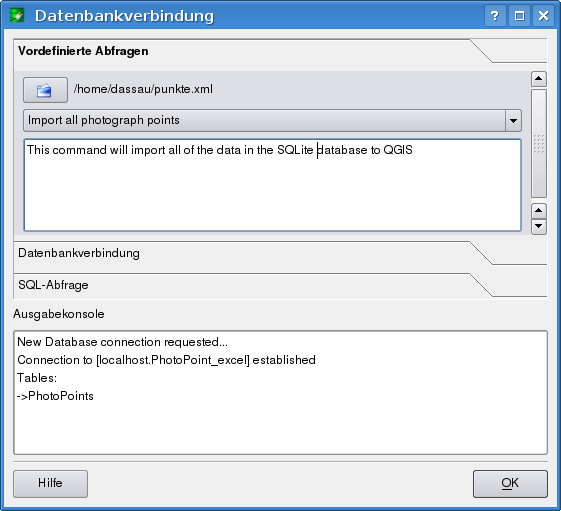
\includegraphics[clip=true, width=10cm]{evispredefined}
%\end{center}
%\end{figure}

\begin{figure}[ht]
   \begin{center}
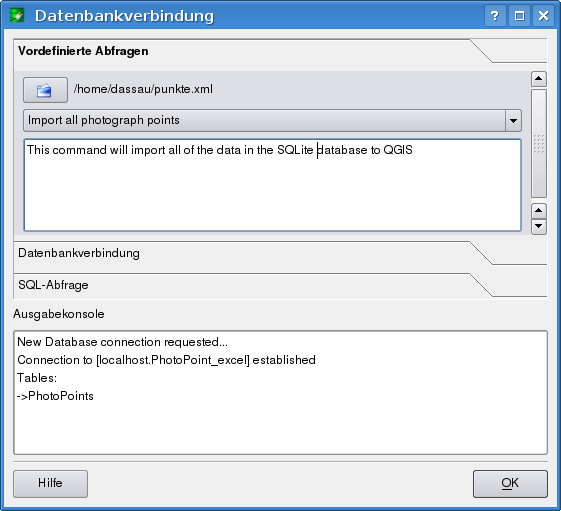
\includegraphics[clip=true, width=8cm]{evispredefined}
\caption{\label{evispredefined}Onglet de requêtes prédéfinies \emph{eVis} \nixcaption}
\end{center}
\end{figure}

%\begin{itemize}
%\item[Open Query File :] Launches the \og Open File\fg  file browser to search for the XML file
%holding the predefined queries.
%\item[Predefined Queries :] A dropdown list with all of the queries defined by the
%predefined queries XML file.
%\item[Query description :] A short description of the query. This description is from the
%predefined queries XML file.
%\item[Console Window :] The console window where messages related to processing are
%displayed.
%\item[Help :] Displays the on line help.
%\item[OK :] Closes the main \og Database Connection\fg  window.
%\end{itemize}

\begin{description}
\item[Ouvrir le fichier :] Lance un explorateur de fichier pour sélectionner le fichier contenant les requêtes au format XML.
\item[Requêtes prédéfinies :] Une liste déroulante affichant toutes les requêtes prédéfinies dans le fichier XML.
\item[Description de la requête :] Une courte description de la requête.
\item[Console :] Console où sont affichés les messages relatifs au déroulement de la connexion.
\item[Aide :] Affiche l'aide en ligne.
\item[OK :] Ferme la fenêtre principale.
\end{description}

%\minisec{XML format for eVis predefined queries}\label{evis_xml_format}
\minisec{Le format XML pour les requêtes d'eVis}\label{evis_xml_format}

%\begin{table}[htp]\index{extension!evis}
%\centering
%\caption{The XML tags read by eVis}\label{tab:evis_xml_tags}\medskip
% \begin{tabular}{|p{1.2in}|p{4.7in}|}
% \hline \textbf{Tag} & \textbf{Description}\\
% \hline query & Defines the beginning and end of a query statement.\\
% \hline shortdescription & A short description of the query that appears in the eVis dropdown
%menu.\\
% \hline description & A more detailed description of the query displayed in the Predefined Query
%text window.\\
% \hline databasetype & The database type as defined in the Database Type dropdown menu in the
%Database Connection tab.\\
% \hline databaseport & The port as defined in the Port textbox in the Database Connection tab.\\
% \hline databasename & The database name as defined in the Database Name textbox in the Database
%Connection tab.\\
% \hline databaseusername & The database username as defined in the Username textbox in the Database
%Connection tab.\\
% \hline databasepassword & The database password as defined in the Password textbox in the Database
%Connection tab.\\
% \hline sqlstatement & The SQL command.\\
% \hline autoconnect & A flag (\og true\fg  or \og false\fg ) to specify if the above tags should be used to
%automatically connect to database without running the database connection routine in the Database
%Connection tab.\\
% \hline
%\end{tabular}
%\end{table}

\begin{table}[ht]\index{extension!evis}
\centering
 \begin{tabular}{|p{3cm}|p{11cm}|}
 \hline \textbf{Balise} & \textbf{Description}\\
 \hline query & Définit le début et la fin d'une requête.\\
 \hline shortdescription & Une courte description qui apparaît dans le menu déroulant.\\
 \hline description & Une description plus détaillée.\\
 \hline databasetype & Le type de base de données tel que définit dans la liste déroulante dans l'onglet de connexion.\\
 \hline databaseport & Le port tel que définit dans la liste déroulante dans l'onglet de connexion.\\
 \hline databasename & Le nom de la base de données tel que définit dans la liste déroulante dans l'onglet de connexion.\\
 \hline databaseusername & Le nom d'utilisateur tel que définit dans la liste déroulante dans l'onglet de connexion.\\
 \hline databasepassword & Le mot de passe tel que définit dans la liste déroulante dans l'onglet de connexion.\\
 \hline sqlstatement & La commande SQL.\\
 \hline autoconnect & Un interrupteur (\og true\fg  or \og false\fg )  pour spécifier si les balises précédentes doivent être utilisées pour ce connceter automatiquement à une base de données sans passer par les routines de connexion de l'onglet.\\
 \hline
\end{tabular}
\caption{les balises XML lues par eVis}\label{tab:evis_xml_tags}
\end{table}

Voici un exemple complet avec 3 requêtes :
{\small
\begin{verbatim}
<?xml version="1.0"?>
<doc>
 <query>
   <shortdescription>Importer tous les points de photographies</shortdescription>
   <description>Cette commande importera toutes les données de la base SQLite vers to QGIS
      </description>
   <databasetype>SQLITE</databasetype>
   <databasehost />
   <databaseport />
   <databasename>C:\textbackslash Workshop/textbackslash
eVis\_Data\textbackslash PhotoPoints.db</databasename>
   <databaseusername />
   <databasepassword />
   <sqlstatement>SELECT Attributes.*, Points.x, Points.y FROM Attributes LEFT JOIN 
      Points ON Points.rec_id=Attributes.point_ID</sqlstatement>
   <autoconnect>false</autoconnect>
 </query>
  <query>
   <shortdescription>Importe les points de photographies "looking across Valley"
   </shortdescription>
   <description>Cette commande n'importera que les points ayant une photographe 
   "looking across a valley"</description>
   <databasetype>SQLITE</databasetype>
   <databasehost />
   <databaseport />
   <databasename>C:\Workshop\eVis_Data\PhotoPoints.db</databasename>
   <databaseusername />
   <databasepassword />
   <sqlstatement>SELECT Attributes.*, Points.x, Points.y FROM Attributes LEFT JOIN 
      Points ON Points.rec_id=Attributes.point_ID where COMMENTS='Looking across 
      valley'</sqlstatement>
   <autoconnect>false</autoconnect>
 </query>
 <query>
   <shortdescription>Importe les points mentionnant "limestone"</shortdescription>
   <description>This command will import only points that have photographs that
   mention "limestone" to \qg</description>
   <databasetype>SQLITE</databasetype>
   <databasehost />
   <databaseport />
   <databasename>C:\Workshop\eVis_Data\PhotoPoints.db</databasename>
   <databaseusername />
   <databasepassword />
   <sqlstatement>SELECT Attributes.*, Points.x, Points.y FROM Attributes LEFT JOIN 
      Points ON Points.rec_id=Attributes.point_ID where COMMENTS like '%limestone%'
      </sqlstatement>
   <autoconnect>false</autoconnect>
 </query>
</doc>
\end{verbatim}}